\pdfoptionpdfminorversion=7
\documentclass[sigconf, table]{acmart}


\usepackage{comment}
\usepackage{graphicx}
\usepackage{csquotes}
\usepackage{balance}
\usepackage{setspace}

\usepackage{listings}
\usepackage{subcaption}

\usepackage{standalone}

\lstset{ %
language=C++,                % choose the language of the code
basicstyle=\ttfamily\footnotesize,       % the size of the fonts that are used for the code
columns=fullflexible,
numbers=left,                   % where to put the line-numbers
numberstyle=\footnotesize,      % the size of the fonts that are used for the line-numbers
stepnumber=1,                   % the step between two line-numbers. If it is 1 each line will be numbered
numbersep=5pt,                  % how far the line-numbers are from the code
%backgroundcolor=\color{codeBG3},  % choose the background color. You must add \usepackage{color}
showspaces=false,               % show spaces adding particular underscores
showstringspaces=false,         % underline spaces within strings
showtabs=false,                 % show tabs within strings adding particular underscores
frame=single,           % adds a frame around the code
tabsize=2,          % sets default tabsize to 2 spaces
captionpos=b           % sets the caption-position to bottom
breaklines=true,        % sets automatic line breaking
breakatwhitespace=false,    % sets if automatic breaks should only happen at whitespace
keywordstyle=\color{blue},       % keyword style
  %language=Octave,                 % the language of the code
  otherkeywords={SearchVar,MV,TSS,tileExpr,Search,tFunc...},           % if you want to add more keywords to the set
  numberstyle=\tiny\color{black}, % the style that is used for the line-numbers
  rulecolor=\color{black},
escapeinside={<@}{@>}
}
\definecolor{ForestGreen}{RGB}{34,139,34}
\newcommand{\todo}[1]{{\textcolor{red}{{\tt{TODO:}}\,\,#1 }}}
\newcommand{\nc}[0]{\todo{cite}}
\newcommand{\an}[1]{{\textcolor{blue}{Author's Note: #1}}}
\newcommand{\ttt}[1]{{\texttt{#1}}}

\newcommand{\FormatDecisions}[0]{{\texttt{FormatDecisions}}~}
\graphicspath{{.}{ScoreValidity}}

\usepackage[subtle]{savetrees}

\title{Something about data layouts}


% \author{Brandon Neth}
% \affiliation{%
% 	\institution{University of Arizona}
% 	\city{Tucson}
% 	\state{AZ}
% 	\country{USA}}
% \email{brandonneth@email.arizona.edu}

% \author{Thomas R.W. Scogland}
% \affiliation{
% 	\institution{Lawrence Livermore National Laboratory}
% 	\city{Livermore}
% 	\state{CA}
% 	\country{USA}}

% \author{Bronis R. de Supinski}
% \affiliation{
% 	\institution{Lawrence Livermore National Laboratory}
% 	\city{Livermore}
% 	\state{CA}
% 	\country{USA}}

% \author{Michelle Mills Strout}
% \affiliation{%
% 	\institution{University of Arizona}
% 	\city{Tucson}
% 	\state{AZ}
% 	\country{USA}}




\begin{document}

\begin{abstract}
In a world of ever-increasing diversity of computing platform, performance portability is of critical importance. 
Especially in high performance computing contexts, the portability of optimizations balancing parallelism and data movement are key. 
Such optimization portability was developed in RAJALC, an extension of RAJA incorporating the loop chain abstraction.
This work created an inter-loop context for the purpose of schedule optimizations like loop fusion and overlapped tiling.
While RAJALC enabled the portable specification of complex schedule changes, it left unleveraged a significant factor on performance: data layouts.
Manipulating the layout of data in memory between computations can provide major performance benefits, but like scheduling optimizations can be laborious to implement and lack portability. 
\todo{This work fixes this using features of RAJA (layout policies and decision objects)}.
First, we present an interface for declaring data layout changes between computations in a loop chain. 
Second, we present an automated layout decider that selects optimal data layouts based on performance estimations.
These systems work together, meaning the decider \enquote{fills in} the layout choices not made by the user.
This allows the user to specify as much or as little of the layout information as they please and still get the performance benefits of changing data layouts.  
We evaluate our system on \todo{what}, where it achieves \todo{what}.
\end{abstract}

\maketitle

\section{Introduction}
\todo{Motivate the problem of performance portability, different layouts for different systems, sometimes the transofrmation is worth it sometimes it isnt, etc}

\section{RAJA and RAJALC}

\todo{INtroduce RAJA and RAJALC. kernel objects, symbolic evaluation, delay between specification and execution.}

We use a variety of components of RAJA and RAJALC to enable automatic data format transformations. This section reviews how a computation is described in RAJA as well as the RAJALC extensions used in this work. 

The foundational elements of RAJA are the execution constructs \verb.forall. and \verb.kernel.. 
These constructs separate the specification of the computation from the specification of its schedule. 
The user provides three pieces of information when using these constructs. 
First, they provide the execution policy. 
This describes the structure of a loop, including schedule choices at each nesting level. 
Second, they provide a tuple of iterators describing the loop bounds. 
Third, they provide a lambda function describing the body of the loop.
While the execution constructs immediately execute the computation they describe, RAJALC introduced wrapper objects that enable the computations to be analyzed and transformed before execution. 
The \verb.make_kernel. function seen at the end of Listing~\ref{MatMulTraversalOrder} creates one such kernel object.

RAJA also provides an array wrapper class called a View.
The View object has a number of capabilities that make it a valuable tool within RAJA codes.
First, Views use the call operator to perform memory accesses. 
By overloading this call operator for symbolic iterator types, RAJALC enabled the runtime symbolic evaluation of kernels that use Views.
RAJALC used the access information gathered from symbolic evaluation to ensure the correctness of its scheduling optimizations.
This work uses RAJALC's runtime symbolic evaluation to inform our performance model \todo{forward reference to where its discussed}.

Second, Views fully parameterize their underlying data formats with the Layout object.
Consider a programmer who wants to switch their data from row-major to column-major. 
Without Views, every access to their data \verb.A[i][j]. has to be changed to \verb.A[j][i]. \textit{and} the definition of the array needs to be changed. 
This is prohibitively expensive, especially when the programmer does not yet know the performance impact of such a decision.
With Views however, the only change the programmer needs to make is to the View's definition: The layout permutation changes from $(0,1)$ to $(1,0)$.


\section{Data Formats in RAJA}

Throughout a computation, different parts of the computation access data in different orders.
For example, \todo{explain 3MM or something}.
Because different formats are optimal for different kernels, this creates an opportunity for optimization. 

However, RAJA's built-in support for changing data layouts is minimal. 
While Views can be instatiated with different layouts, changing the layout of an existing View is not as simple.
This is because changing layouts also requires reordering the underlying data to match the new layout. 
To implement such a layout change by hand requires the programmer to allocate a new temporary array, copy the data from the View to the temporary array in the right order, copy the data \textit{back} to the memory in the View, and then finally update the View's layout object.

\todo{Explain how layouts work}

\section{\texttt{FormatDecisions}: User Specification of Data Format}

This work forwards the goal of enabling portable, declarative data optimizations begun by RAJALC.
While RAJALC tackled the problem of scheduling optimizations, we target making data format changes between computations. 
The new \verb.FormatDecisions. object is the central component of our system. 
Its instantiation takes a tuple of references to Views that are possible targets of format changes and the kernel objects that constitute the whole computation.
Two methods are used to register desired formats: \verb.set_format_before. and \verb.set_format_after..
Both take the View to be reformated, the desired format, and the computation before or after which the desired format should be used.
Once all the format choices are registered, the complete computation with the desired format conversions is generated using the \verb.finalize. method.


\begin{figure}
\begin{lstlisting}
auto knl1 = make_kernel<KPOL>(segs1, [=](auto i0, auto i1, auto i2) {
	E(i0, i1) += A(i0, i2) * B(i2, i1);
});
auto knl2 = make_kernel<KPOL>(segs2, [=](auto i0, auto i1, auto i2) {
	F(i0, i1) += C(i0, i2) * D(i2, i1);
});
auto knl3 = make_kernel<KPOL>(segs3, [=](auto i0, auto i1, auto i2) {
	G(i0, i1) += E(i0, i2) * F(i2, i1);
});

auto decisions = format_decisions(tie(B,D,F), knl1, knl2, knl3);

decisions.set_format_before(B, {{1,0}}, knl1);
decisions.set_format_before(D, {{1,0}}, knl2);

decisions.set_format_before(F, {{0,1}}, knl1);
decisions.set_format_after(F, {{1,0}}, knl2);

auto computation = decisions.finalize();
computation();
\end{lstlisting}
\end{figure}

\todo{Explain how \texttt{FormatDecisions} object works for a computation}

\section{Traversal Order}

In this section, we describe how RAJALC estimates the cost of a particular layout choice and how cost metrics are reused where possible.
When deciding between possible layout choices for a kernel, RAJALC determines the traversal order of each access in the kernel.
An access' traversal order describes which iterators in a kernel traverse which dimensions of a view, based on the depth of the iterator and the strides of the dimensions.

\subsection{Deriving the Traversal Order}

Given an $n$-dimensional kernel that accesses a $d$-dimensional view, there are $n! * d!$ different possible combinations of kernel policy and data layout. 
Estimating the cost of all of these choices separately for each access in a computation is prohibitively expensive, especially using any sort of dynamic benchmarking. 
However, the traversal order of an access compresses the kernel policy and data layout into a single reusable feature that accurately predicts relative performance.


\begin{figure}
\begin{lstlisting}[
	caption={Two kernels implementing matrix multiplication using different kernel policies.},
	label={MatMulTraversalOrder}]
View2D A(A_data, layout_01);
View2D B(B_data, layout_10);
View2D C(C_data, layout_01);

auto loop_body = [=](auto i0, auto i1, auto i2) {
	C(i0,i1) += A(i0,i2) * B(i2,i1);
}

using Policy_012 = KernelPolicy<
	statement::For<0, loop_exec,
    	statement::For<1, loop_exec,
	  		statement::For<2, loop_exec,
			  	statement::Lambda<0>
	  		>
		>
  	>
>;
using Policy_201 = KernelPolicy<
	statement::For<2, loop_exec,
    	statement::For<0, loop_exec,
	  		statement::For<1, loop_exec,
			  	statement::Lambda<0>
	  		>
		>
  	>
>;

auto knl1 = make_kernel<Policy_012>(bounds, loop_body);
auto knl2 = make_kernel<Policy_201>(bounds, loop_body);
\end{lstlisting}
\end{figure}

Listing~\ref{MatMulTraversalOrder} shows two implementations of a matrix multiplication using different kernel policies and involving views using different data layouts.
Deriving the traversal order for an access requires the extraction of three values: the policy order, the layout order, and the argument order. 
For the access to \verb.C. in \verb.knl1., the policy order is $(0,1,2)$, the layout order is $(0,1)$, and the argument order is $(0,1)$. 
In contrast, for the access to \verb.B. in \verb.knl2., the policy order is $(2,0,1)$, the layout order is $(1,0)$, and the argument order is $(2,1)$. 

With these values in hand, we can derive the traversal order, using the access to \verb.B. in \verb.knl2. as a running example. 
We start with the argument order $(2,1)$.
The first step is to normalize the policy order.
This step gives us the answer to the question: \enquote{What access has the same traversal order when the policy order is monotonically increasing (the normal policy order)?}
This is calculated using the following: \verb,[policy_order.indexof(arg) for arg in arg_order],. 
The index of $2$ in the policy is $0$, and the index of $1$ in the policy is $2$, so our intermediate value is $(0,2)$. 

The second step is to permute this intermediate value based on the data layout. 
We apply the layout permutation $(1,0)$ to our intermediate value $(0,2)$ to get our traversal order $(2,0)$. 
This traversal order tells us that in the access to \verb.B. in \verb.knl2., the dimension of \verb.B. with the largest stride is traversed by the iterator at nesting depth 2 (the innermost iterator) and the dimension of \verb.B. with the smallest stride is traversed by the iterator at nesting depth 0 (the outermost iterator). 

\subsection{Traversal Order as a Performance Metric}

Our claim is that the traversal order of an access is an accurate predictive metric for the relative performance of a layout choice. 
We support this claim empirically using performance data from three microbenchmarks.
For each microbenchmark, we record the 5-run average execution time of every combination of kernel policy and data layout. 
These execution times are then grouped by traversal order.
If our claim is valid, then the execution times for each traversal order will cluster and the groups of execution times will not overlap.

Microbenchmark 1 is an access to a 3-dimensional view in a 3-dimensional loop. 
Microbenchmark 2 is an access to a 2-dimensional view in a 3-dimensional loop, as in a matrix multiplication.
Microbenchmark 3 is an access to a 3-dimensional view in a 4-dimensional loop.


\begin{figure}
% 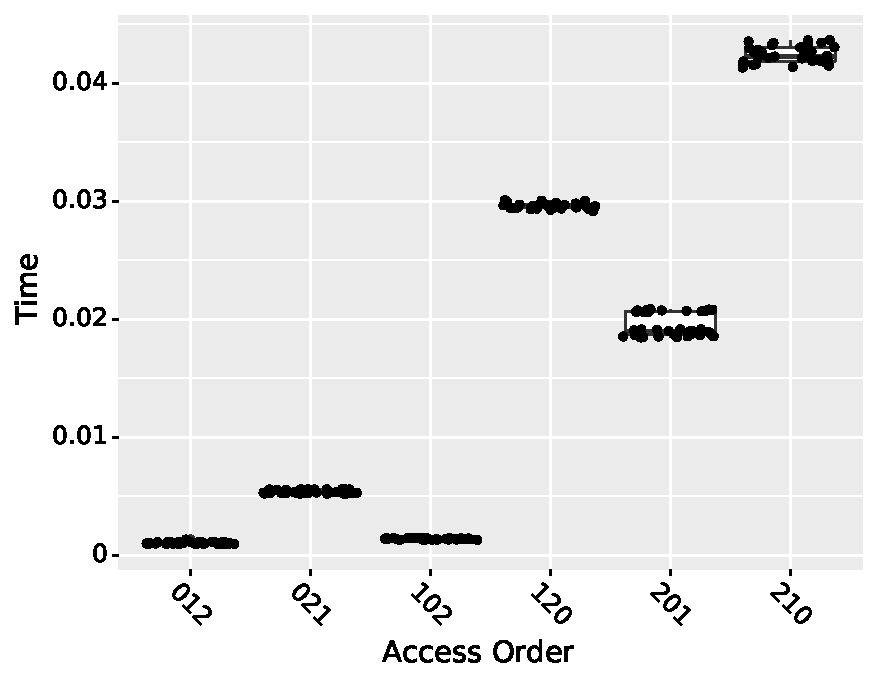
\includegraphics{benchmark1_boxplot.pdf}
\caption{Execution times for 3-dimensional loop accessing 3-dimensional view, grouped by traversal order.}
\label{TraversalBenchmark1}
\end{figure}

\begin{figure}
	% 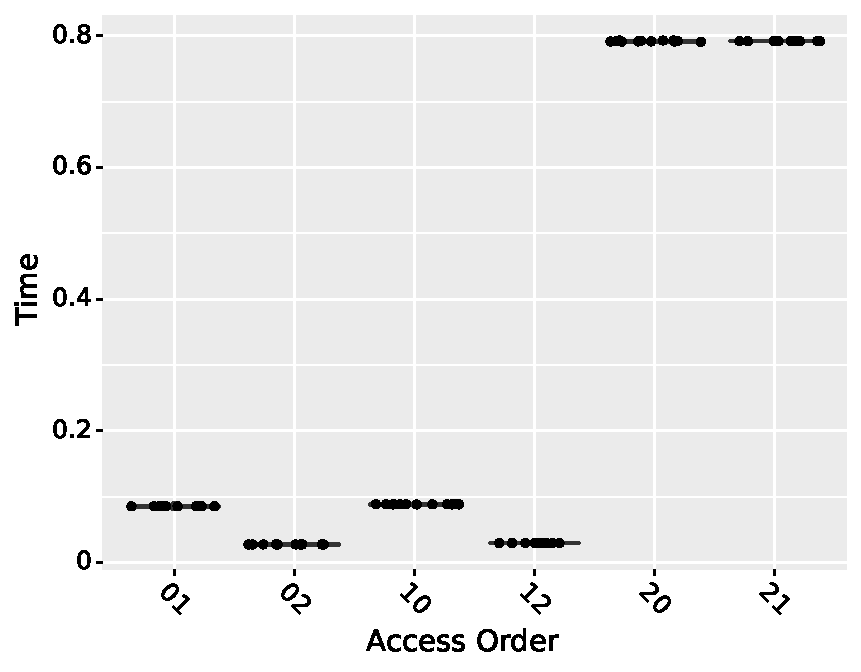
\includegraphics{benchmark2_boxplot.pdf}
	\caption{Execution times for 3-dimensional loop accessing 2-dimensional view, grouped by traversal order.}
	\label{TraversalBenchmark2}
\end{figure}

\begin{figure}
	% 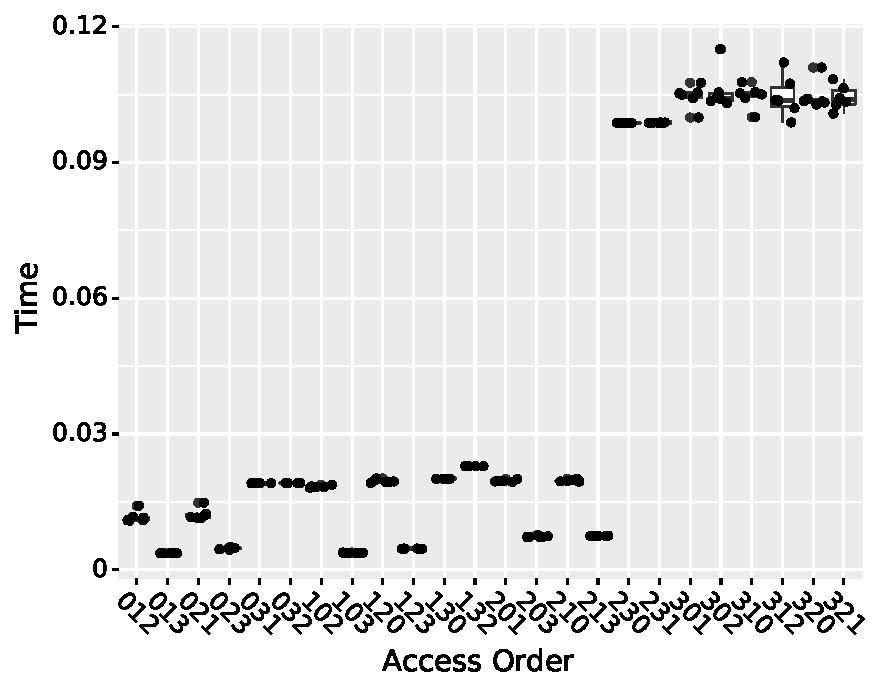
\includegraphics{benchmark3_boxplot.pdf}
	\caption{Execution times for 4-dimensional loop accessing 3-dimensional view, grouped by traversal order.}
	\label{TraversalBenchmark3}
\end{figure}

Figure~\ref{TraversalBenchmark1} shows the execution times for the different traversal orders for microbenchmark 1. 
With the exception of traversal order $(2,1,0)$, the traversal orders show good clustering.
\todo{explanation for why the $(2,1,0)$ ones don't cluster as much}
Also, the six possible traversal orders show good differentiation, with the exception of $(0,1,2)$ and $(1,0,2)$. 
This is likely because the bulk of the performance improvement comes from the innermost loop in a nest traversing the stride 1 dimension of the data.



Figure~\ref{TraversalBenchmark2} shows the execution times for the different traversal orders for microbenchmark 2. 
While the traversal orders for this microbenchmark are all highly clustered, they are less differentiated from one another. 
For example, we see that the orders $(0,2)$ and $(1,2)$ have similar performance, as do $(2,0)$ and $(2,1)$. 
The similarity in performance is again attributable to the influence of the position of the innermost loop iterator. 



Figure~\ref{TraversalBenchmark3} shows the execution times for the different traversal orders for microbenchmark 3. 
A similar pattern as the previous microbenchmarks emerges here: grouping based on the position of the innermost iterator. 

The major benefit of using traversal order as a performance metric is its reusability. 
Because it condenses the policy, the layout, and the arguments used in the access into a single metric, the same benchmarking results can be used to estimate the cost of all three accesses within a matrix multiplication. 
Similarly, the benchmarking results for traversal orders gathered for one computation can be reused when modeling another computation.

\section{A Performance Model for Data Format}

\todo{explain how we use the traversal order information to build up a model and choose layouts and generate the computation}

\section{Evaluation}

\todo{Where we evaluated}

We evaluate our contribution on three codes: the polybench suite\nc, Kripke\nc, and miniWeather\nc.


\subsection{Evaluation Metrics}
When evaluating our systems, we consider a number of metrics. 
First,  we measure the source lines of code (SLOC) added, removed, and changed to implement layout changes by hand and using our \FormatDecisions interface.
Second, we measure the relative performance improvement between implementing layout changes by hand and using \FormatDecisions. 
This result shows the cost of modeling overhead.
Third, we measure the accuracy of our model on its own by determining the rank of its choices among all possible choices.
\todo{The explanation of the model accuracy measurement needs work.} 

\subsection{Case Study 1: Polybench}

Our first evaluation targeted the kernels within the Polybench suite. 
Polybench contains 30 numerical computations in total. 
Of those 30, 13 have good traversal orders for all multi-dimensional accesses, one uses only 1D data, and one uses external functions that inhibit RAJALC's symbolic evaluation.
This leaves 15 benchmarks to evaluate.

We evaluated the performance of three variants of the benchmarks.
The first variant, \verb.RAJA_OpenMP., is the original RAJA implementation of the kernel.
The second variant, \verb.Hand_Layout., implements the layout changes by hand.
The third variant, \verb.Auto_Layout., implements the layout changes using our contribution.



\todo{This table is temporary.}
\begin{figure*}
\begin{tabular}{ll}
Benchmark   & Inclusion \\
2mm         & Yes          \\
3mm         & Yes          \\
adi         & Yes          \\
atax        & No, accesses to A are in-order.          \\
bicg        & No, accesses to A are in-order.          \\
cholesky    & No, accesses to A are in-order.          \\
correlation & Yes          \\
covariance  & Yes          \\
deriche     & No, accesses to all multi-dimensional data are in-order.          \\
doitgen     & Yes          \\
durbin      & No, all 1D data.          \\
fdtd-2d     & No, accesses to all multi-dimensional data are in-order.           \\
floyd-warshall & No, accesses are in order \\
gemm        &  No, accesses are all in order         \\
gemver      & Yes          \\
gesummv     & No, accesses are all in order          \\
gramschmidt & Yes          \\
heat-3d     & No, accesses are all in order            \\
jacobi-1D   & No, accesses are all in order           \\
jacobi-2D   & No, accesses are all in order           \\
lu          & Yes         \\
ludcmp      & Yes          \\
mvt         & Yes          \\
nussinov    & No, too much control flow and function calls          \\
seidel      & No, accesses are all in order           \\
symm        & Yes          \\
syr2k       & Yes          \\
syrk        & Yes          \\
trisolv     & No, accesses are all in order           \\
trmm        & Yes         
\end{tabular}
\caption{Polybench benchmarks}
\end{figure*}


\subsection{Case Study 2: miniWeather}

\subsection{Case Study 3: Kripke}


\section{Conclusion}


\end{document}
